

\documentclass[12pt]{report}
\usepackage[utf8]{inputenc}
\usepackage[russian]{babel}
\usepackage[14pt]{extsizes}
\usepackage{listings}
\usepackage{graphicx}
\usepackage{amsmath,amsfonts,amssymb,amsthm,mathtools} 
\usepackage{pgfplots}
\usepackage{filecontents}
\usepackage{float}
\usepackage{indentfirst}
\usepackage{eucal}
\usepackage{enumitem}
%s\documentclass[openany]{book}
\frenchspacing

\usepackage{titlesec}
\titleformat{\section}
{\normalsize\bfseries}
{\thesection}
{1em}{}
\titlespacing*{\chapter}{0pt}{-30pt}{8pt}
\titlespacing*{\section}{\parindent}{*4}{*4}
\titlespacing*{\subsection}{\parindent}{*4}{*4}

\usepackage{indentfirst} % Красная строка

\usetikzlibrary{datavisualization}
\usetikzlibrary{datavisualization.formats.functions}

\usepackage{amsmath}

\usepackage{amssymb}

% Для листинга кода:
\lstset{ %
	language=lisp,                 % выбор языка для подсветки (здесь это С)
	texcl=true,
	extendedchars=\true,
	basicstyle=\small\sffamily, % размер и начертание шрифта для подсветки кода
	numbers=left,               % где поставить нумерацию строк (слева\справа)
	numberstyle=\tiny,           % размер шрифта для номеров строк
	stepnumber=1,                   % размер шага между двумя номерами строк
	numbersep=5pt,                % как далеко отстоят номера строк от подсвечиваемого кода
	showspaces=false,            % показывать или нет пробелы специальными отступами
	showstringspaces=false,      % показывать или нет пробелы в строках
	showtabs=false,             % показывать или нет табуляцию в строках
	frame=single,              % рисовать рамку вокруг кода
	tabsize=2,                 % размер табуляции по умолчанию равен 2 пробелам
	captionpos=t,              % позиция заголовка вверху [t] или внизу [b] 
	breaklines=true,           % автоматически переносить строки (да\нет)
	breakatwhitespace=false, % переносить строки только если есть пробел
	escapeinside={\#*}{*)},  % если нужно добавить комментарии в коде
	%inputencoding=utf8x,
	%extendedchars=\true
}



\usepackage[left=2cm,right=2cm, top=2cm,bottom=2cm,bindingoffset=0cm]{geometry}
% Для измененных титулов глав:
\usepackage{titlesec, blindtext, color} % подключаем нужные пакеты
\definecolor{gray75}{gray}{0.75} % определяем цвет
\newcommand{\hsp}{\hspace{20pt}} % длина линии в 20pt
% titleformat определяет стиль
\titleformat{\chapter}[hang]{\Huge\bfseries}{\thechapter\hsp\textcolor{gray75}{|}\hsp}{0pt}{\Huge\bfseries}


% plot
\usepackage{pgfplots}
\usepackage{filecontents}
\usepackage[unicode, pdftex]{hyperref}
\usetikzlibrary{datavisualization}
\usetikzlibrary{datavisualization.formats.functions}

 
\begin{document}

\chapter{Теоретическая часть}





\section{Общее}
Конъюнкция, дизъюнкция, отрицание  --  базовые функции матлогики. Предикат - логическая функция. Базис пролога -- матлогика.

В прологе используется символьная обработка. Декларативная методология. Мы описываем систему знаний из предметной области. Потом задаем вопрос, но хотим получить не только да/нет, но и как (как побочный эффект)? Не запрещено использовать символы. 


Запросы могут быть конъ или дизъ, но нам будут запрещать их использовать

что такое декларативно? (интернет - Декларативное программирование — это парадигма, при которой описывается желаемый результат, без составления детального алгоритма его получения.)









\section{Терм}

Терм - основной элемент языка Prolog. Терм – это:

\begin{enumerate}
	\item константа -- ква(используется для обозначения объекта/процесса предметной области или для обозначения конкретного отношения): 
	\begin{itemize}
		\item число (целое, вещественное),
		\item cимвольный атом -- комбинация символов латинского алфавита, цифр и ’\_’ (символа подчеркивания), начинающаяся со строчной буквы,
		\item строка -- последовательность символов, заключенных в кавычки;
	\end{itemize}
	\item переменная:
	\begin{itemize}
		\item именованная -- комбинация символов латинского алфавита, цифр и ’\_’, начинающаяся с прописной буквы или символа подчеркивания, может связываться с различными объектами (конкретизироваться),
		\item анонимная  - обозначается символом ’\_’, не может быть связана со значением;
	\end{itemize}
	\item составной терм (составное тело) -- средство фиксации информации о том, что между объектами существует определенная связь. Синтаксически представляется так: f(t1, t2, …, tm), где f -  главный (тк внутри мб другие) функтор -- символьная константа, обозначающая имя отношения между объектами; t1, t2, …, tm – термы (в том  числе  и составные), являющиеся аргументами (арность -- число аргументов).
\end{enumerate}



student(ivanov, mgtu) - константы
student(X, mgtu) -- группа студентов из мгту. В момент фиксации система не знает, что такое X
student(ivanov, mgtu) и student(ivanov) -- для системы разные запросы.

Первые аргуметы считаются как объекты одной природы, вторые - другой. Только мы определям смысл.









\section{Переменные}

Зачем нужны переменные -- для повышения уровня абстракции. Чем больше переменных, тем выше уровень абстракции.

Именованная переменная представляет собой комбинацию символов латинского алфавита, цифр и ’\_’, начинающуюся с прописной буквы или символа подчеркивания. В процессе выполнения программы именованные переменные могут связываться с различными объектами – конкретизироваться. Именованная переменная является уникальной в рамках предложения. В разных предложениях может использоваться одно имя переменной для обозначения разных объектов.

Анонимная  переменная обозначается символом ’\_’. Она не может быть связана со значением. Любая анонимная переменная уникальна.

(Уникальность: именованная переменная уникальна в рамках одного предложения. Анонимная переменная уникальна всегда.)

(Именованные) Переменные предназначены для передачи информации «во времени (за конечное число шагов получить результат) и пространстве (передача значений через параметры)». Для этого в какой-то момент переменная дб конкретизирована каким-то значением. Но это может  быть ошибочным, есть механизм отказа (отката), реконкретизировать переменную. В момент фиксации система не знает, какой объект представляет переменная. Во многих языках последовательность действий при работе с переменными такая: задать значение переменной, а затем работать с самой переменной. В прологе же особый способ работы с переменными. Методом проб и ошибок. Цель -- подтвердить истинность вопроса с помощью бз. 

Установление значения длля переменной не связано с понятием типа  (по указателям). 

Анонимные переменные система не конкретизирует значениями.


Именованная переменная входит в факты и правила с квантором всеобщности, а в вопрос с квантором существования.








\section{Что собой представляет программа на языке пролог?}

\textbf{Программа на Prolog} представляет собой базу знаний и вопрос. 

\begin{itemize}
	\item \textbf{База знаний} состоит из предложений -- фактов и правил, -- используя которые программа выдает ответ на вопрос. Каждое предложение  должно заканчиваться точкой.
	\begin{itemize}
		\item \textbf{Правило} имеет вид: A :- B1, ... , Bn, где A -- заголовок правила (составной терм, который содержит знание); B1, ... , Bn - тело правила (составные термы, которые содержат условия истинности этого знания), символ $":-"$ -- это специальный символ-разделитель. Заголовоок - фиксацияя знания о том, что между аргументами мб истинная связь
		\item \textbf{Факт} -- это частный случай правила -- предложение, в котором отсутствует тело (то есть тело пустое).
	\end{itemize}
	\item \textbf{Вопрос} -- ??это частный случай правила -- предложение, которое состоит только из тела. Используется, чтобы определить, выполняется ли некоторое отношение между описанными в программе объектами. Система рассматривает вопрос как цель, к которой (к истинности которой) надо стремиться. Ответ на вопрос может оказаться логически положительным или отрицательным, в зависимости от того, может ли быть достигнута соответствующая цель.
\end{itemize}

Вопросы и правила (факты) без переменных -- основные (предназначены для описания отношений, формирования базы знаний), с переменными -- неосновные (для поиска ответа в базе знаний)


В базе знаний нет порядка.

В момент фиксации знания (если еще оно с условием, переменными)  --  условная истина.


Алгоритм унификации - единственный алгоритм доказательства. Многократно запускается (в какой момент?)










\section{Структура программы на Prolog}

Программа на Prolog состоит из следующих разделов, каждый из которых начинается со своего заголовка.

\begin{itemize}
	\item директивы компилятора — зарезервированные символьные константы,
	\item CONSTANTS — раздел описания констант,
	\item DOMAINS — раздел описания доменов,
	\item DATABASE — раздел описания предикатов внутренней базы данных,
	\item PREDICATES — раздел описания предикатов,
	\item CLAUSES — раздел описания предложений базы знаний,
	\item GOAL — раздел описания внутренней цели (вопроса).
\end{itemize}

В программе не обязательно должны быть все разделы.























\section{Как реализуется программа на Prolog? Как формируются результаты работы программы?}

Ответ: Программа на Prolog представляет собой базу знаний и вопрос. База знаний состоит из предложений -- фактов и правил, которые задают истинные знания. Ответ на вопрос может оказаться логически положительным или отрицательным, в зависимости от того, может ли быть достигнута соответствующая цель. 

Вопрос рассматривается системой как цель: найти возможность, исходя из базы знаний, ответить «Да» на поставленный вопрос . Вариантов ответить «Да» на может быть несколько. При поиске ответа рассматриваются альтернативные варианты и находятся все возможные решения (методом проб и ошибок) - множества значений переменных, при которых на поставленный вопрос можно ответить - «Да».


Для выполнения логического вывода используется механизм унификации, встроенный в систему.\\















\chapter*{Лекция 2}

Алгоритм унификации - единственный алгоритм доказательства. Многократно запускается (в какой момент?)
<3





\section*{процедурные и декларативные особенности пролога}

Чтобы ответить на вопрос, надо подобрать знание, сравивая вопрос с знаниями.  И то, и то -- составной терм. Сравнивает по 2 состсавных терма по формальному признаку. Порядок формально установлен  сверху вниз.

Если есть переменная и в вопросе, и в формулировке знания (а если еще и на одной позиции)





\section{Что такое предикат в матлогике (математике)?}

Предикат в математической логике -- это (логическая) функция со множеством значений {0, 1} (истина/ложь), определенная на некотором множестве параметров. Предикат называю n-арным, если он определен на n-ой декартовой степени множества М. Таким образом, каждый набор параметров характеризуется либо как «истинный», либо как «ложный».


\section{Что описывает предикат в Prolog?}

Процедура -- совокупность правил (описывающих определенное отношение), заголовки которых имеют одинаковые главнаые функторы, одинаковое число аргументов, обозначающих объекты одной природы (не про память). 

Это одно знание, которое мб зафиксировано через несколько. Структура знания описывается в разделе предикатов. 

??Предикат -- отношение, определяемое процедурой. Таким образом, предикат в Prolog описывает отношение между аргументами процедуры. 








\section*{подстановки и примеры терма}


Дан неосновной термы: A(X1, ..., Xn), Xi -- переменные.

Чтобы подбирать значения переменных нужно построить подстановку. Прнято обозначать $\Theta$

Подстановкой называется множество пар  вида {xi=ti}, где xi -- переменная, ti  -- терм, не содержащий переменных (ti -- значение для переменной xi). \\

Применение подстановки заключается в замене каждого вхождения переменной $x_i$ на соответствующий терм. 

Пусть $\Theta: {X}_{1} = {t}_{1} , {X}_{2} = {t}_{2},… , {X}_{n} = {t}_{n}$ -- подстановка. Тогда результат применения подстановки к терму обозначается $A\Theta$. \\


Терм B называется примером терма A, если существует такая подстановка $\Theta$, что $B = A\Theta$.

Терм С называется общим примером термов А и B, если существуют такие подстановки $\Theta_1$ и $\Theta_2$, что $С = A\Theta_1$ и $С = B\Theta_2$.


A = plus(1, 2, z)
plus(X, Y, 3)



В процессе выполнения программы система, используя встроенный алгоритм унификации, пытается обосновать возможность истинности вопроса, строя подстановки и примеры термов (вопроса и формулировки знания), используя базу знаний. Построение и подстановки производится путём конкретизации переменных. Сами термы хранятся в стеке.




\section*{Простейшие правила логического вывода}


\textbf{Правила вывода} -- утверждения о взаимосвязи между допущениями, которые с позиции исчисления предикатов верны всегда. Возможны 4 варианта:

\begin{enumerate}
    \item факты основные (квантор существования), вопрос основной -- правило: совпадение
    \item факты основные (квантор существования), вопрос неосновной -- правило: обобщение факта
    \item факты неосновные (квантор всеобщности), вопрос основной -- правило: конкретизации факта
    \item факты неосновные (квантор всеобщности), вопрос неосновной -- система должна посстроить пример терма-вопроса и терма-знания (подобрать соответствующие подстановки). Общий пример строится в 2 шага -- сначала конкретизация правила, а потом правило обобщения.
\end{enumerate}





\section*{Унификация терма}

Подбор знания. Назначение -- если сработал, значит для доказательства истинности ответа на вопрос можно использовать знание.

По императивному принципу



\textbf{Унификация} – операция, которая позволяет формализовать процесс логического вывода. С практической точки зрения  - это основной вычислительный шаг, с помощью которого происходят:
\begin{itemize}
	\item двунаправленная передача параметров процедурам (знание в несколько предложений),
	\item неразрушающее присваивание (конкретизация),
	\item проверка условий (доказательство).
\end{itemize}

В процессе работы система выполняет большое число унификаций.  Попытка "увидеть одинаковость" – сопоставимость двух термов, может завершаться успехом или тупиковой ситуацией (неудачей). В последнем случае включается механизм отката к предыдущему шагу.\\



Унифицировать (понять, что это знание подходит для доказательства этого вопроса) два терма. Два терма про одно и то же (T1=T2: = -- принудительный (явный) запуск  унификации)




Два терма унификируются по следующим правилам:

\begin{enumerate}
    \item Если T1 и T2 -- константы: только если они совпадают
    \item Если T1 -- неконкретизированная переменнаяя, а Т2 -- константа или составной терм, не содержащий в качестве аргумента Т1: унификация успешна, а Т1 конкретизируется значением Т2
    \item Если Т1 и Т2 -- неконкретизированные (не имеющие значения) переменные: унификация всегда успешна, причем Т1 и Т2 становятсяя сцеплёнными двумя именами (указателями) одного и того же объекта. \\Если одна из переменных или оин из тером конкретизивуется значением, то второй моментально тоже конкретизируется им же
    \item Если Т1 и Т2 -- составные термы (например, вопрос и заголовок): успешно унифицируются если
    \begin{enumerate}
        \item у Т1 и Т2 одинаковые главные функторы
        \item Т1 и Т2 имеют равные арности
        \item успешно унифицируется каждая пара их  соответствующих компонент
    \end{enumerate}
\end{enumerate}







\section*{Алгоритм унификации}

рабочее поле, стек (для хранения равенств, возможность равенства которых проверяется), результирующая ячейка (динамическая облсьб памяи, в которой накаплливается подставновка)

T1=T2

Начало
\begin{itemize}
	\item Занеси T1=T2
	\item Неудача=0
	\item Пока стек не пус
	\begin{itemize}
		\item Считать из стека в рабочее поле S=T
		\item обработать 
		\begin{itemize}
			\item а)если  S и T -- несовпадающие консаны, то неудача
		\item б) совпадающие константы -- на конец цикла
		\item в) S -- переменная, а T -- терм, содержащий S, то неудача=1 и выход из цикла
		\item г) S -- переменная, а T -- терм, не содержащий S, (для S это возм знач), то отыскать в стеке и результ ячейке все  вхождения S и заменить их на T. Добавить в результирующую ячейку S=T, следующий шаг цикла.
		\item д) S и t составные термы,  им разные функторы или разную арность, то неудача=1 и выхоод из циклы
		\item е) составные термы с одинаковыми функторами и арностями, занести в стек равенства S1=T1, ... Sk=Tks
		\end{itemize}
		\item очистить рабочее поле
		\item конец цикла
	\end{itemize}
\item если неудача=1, то унификация невозможна, иначе -- успешна,  а РЯ содержит подстановку -- эта подстановка называется наиболее общий унификатор. 
\end{itemize}

Терм S называется более общим, чем T, если  T является примером S, а S не является примером T.

Терм S называется наиболее общим примером T1 и T2, если S -- такой их общий пример, который являяется более общим по отношению к любому другому их примеру.

Унификатором двух термов называется подстановка, которая будучи применена к 2 термам даст одинаковый результат.

Наиболее обзим унификатором двух ттермов называется унификаттор, соответсв наиболее обзему примеру двух термов.

Если  2 терма унифицируемы, то сущ единственный (с ттчностью до переименования переменных) наиболее общзий унификатор, а значчит наиболее общий пример.

Алгоритм унификации и строит наиболее общий пример

....



\section{Общая схема согласования целевых утверждений}

Рещение задачи с пом лог прог начинается с задания вопроса G и завершается получением одного из двух результатов: 
\begin{itemize}
	\item Успешного согласования вопроса и программы, а в качестве побочного эффекта будет получена подстановка, которая содержит значения переменных, при которых вопрос является примером программы (или несколько)
	\item Неудача
\end{itemize}

Вычисления с пом конеч лог прог представляет собой пошаговое преобразование исходношо вопроса.

На каждом шаге имеется некоторая конъюнкция целей, выводимость которой следует доказать. Эта конъюнкция целей называется резольвентой (меняется, динамическа) и хранится в виде стека.

Успех достигается тогда, когда резольвента пуста.


Преобразование резольвенты выполняется с помощью преобразования, которое называется редукцией.

Редукцией цели G с пом программы P называется замена цели G телом того правила из P, заголовок которого унифицировался с целью (это правило называется сопоставимым с целью)

Новаяя резольвента выполняется в 2 шага:
\begin{itemize}
	\item  В текущей Р выбирается одна из целей и для нее выполняется редукция.
	\item  К полученной конъюнкции целей применяется подстановка, полученная как наибольший общий унификатор цели и заголовка сопоставленного с ним правила.
\end{itemize}

Если в рез работы алгоритма унификации для редукции был подобран факт, то резольвента уменьшится на одну цель


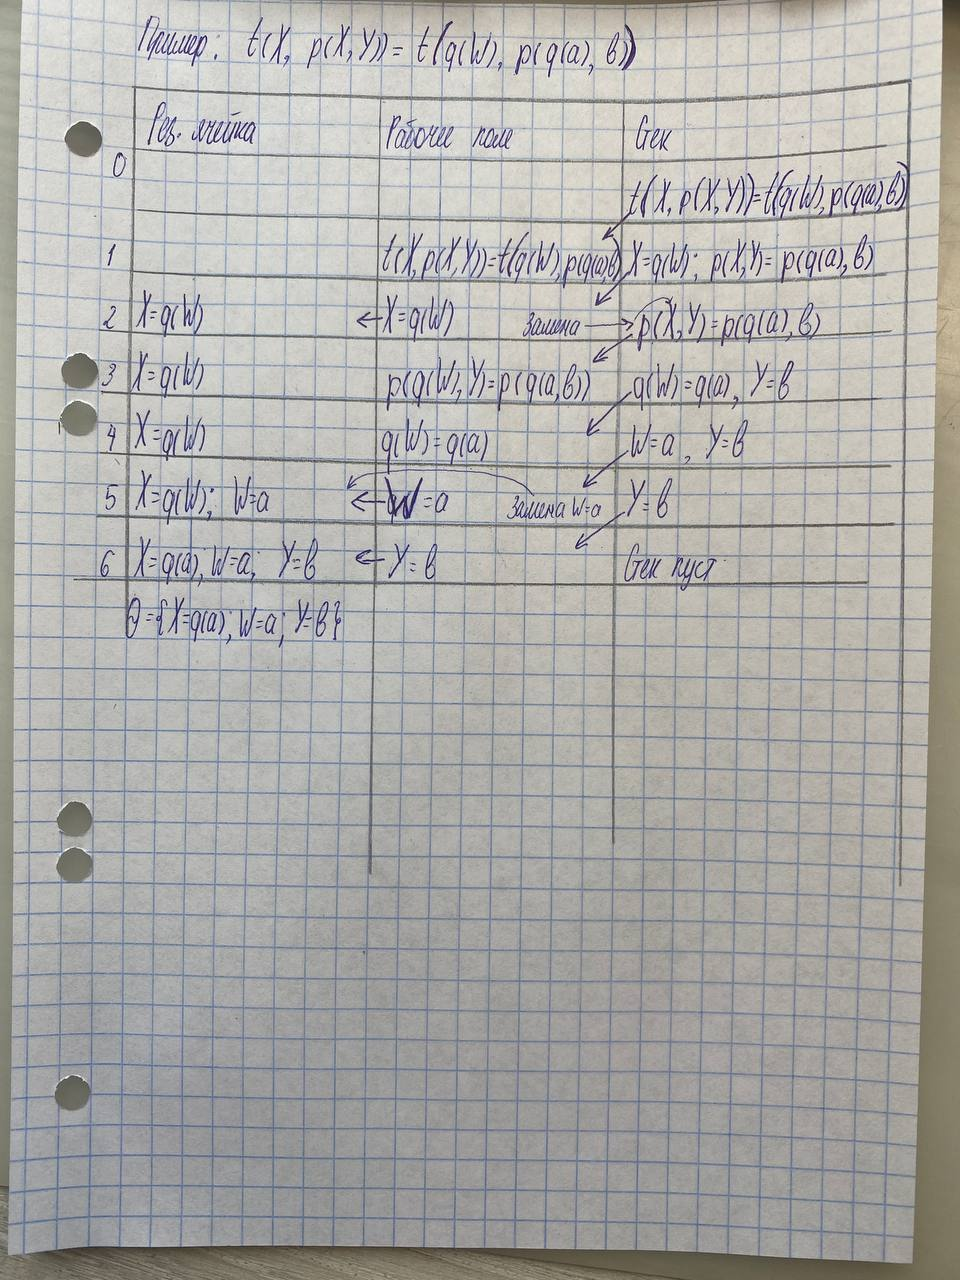
\includegraphics[width=\linewidth]{img/example}


\section{Отсчечение}

Пролог предусматривает возможность отсечения, которая используется для прерывания поиска с возвратом; отсечение обозначается восклицательным знаком (!). Действует отсечение просто: через него невозможно совершить откат (поиск с возвратом).

Отсечение помещается в программу таким же образом, как и подцель в теле правила. Когда процесс проходит через отсечение, немедленно удовлетворяется обращение к cut и выполняется обращение к очередной подцели (если таковая имеется). Однажды пройдя через отсечение, уже невозможно произвести откат к подцелям, расположенным в обрабатываемом предложении перед отсечением, и также невозможно возвратиться к другим предложениям, определяющим обрабатывающий предикат (предикат, содержащий отсечение).

Существуют два основных случая применения отсечения.

Если вы заранее знаете, что определенные посылки никогда не приведут к осмысленным решениям (поиск решений в этом случае будет лишней тратой времени), - примените отсечение, - программа станет быстрее и экономичнее. Такой прием называют зеленым отсечением.
Если отсечения требует сама логика программы для исключения из рассмотрения альтернативных подцелей. Это - красное отсечение.

\chapter{Лекция 3}


Механизм  унификации -- основной, но не единственный шаг.

Резольвенту использует СИСТЕМА, а не унификация. Первое состояние - вопрос. Док-во истинности заключается в преобразовании резольвенты (уже в другой области).

Стек растущий влево

Система исп доп области


\section{механизм отката}


На каждом новом этапе док-ва истинности вопроса может сложиться одна из 3 ситуаций

\begin{itemize}
\item 1) решение (все) найдено -- завершение алгоритма

признаком нового шага является новое состояние резольвенты 

\item 2) имеется некоторое число возможных дальнейших действий, но неизвестно, какое (какой выбор) приблизит к решениям

\item 3) решение не найдено и из данного состояния  невозможен переход в новое (тупиковая ситуация) -- необходим возврат (откат)

\end{itemize}

\section{Дерево поиска решений}
 
Это формализм для исследования возмодных  путей решения.
 
При доказательстве цели G с пом программы P дерево определяется: 

\begin{itemize}
\item  Корень -- вопрос, 
\item  вершины -- резольвенты (конъюнктивная, в виде стека)
\item  ребро -- переход. На ребре записывается подстановка, соотв определенному выбору. Но в каком порядке -- как в бз. Если откат - стрелочка обратно
\item  лист дерева наз успешной вершиной, если резольвента пуста (надо подписать), и безуспешной -- если тупиковая ситуация (нет знания, которое позволяет доказать истинности верхней цели резольвенты)
\end{itemize}

\section{Повышение эффективности работы программы на пролог}

Предикат отсечения (cut):обозначается !,  Отсекает безуспешные ветки поиска решения

Предикат fail  --  принудительно включает механизм отката. Может только вв конце правила по сути


Названияя -- главные функторы (нульместные)

Часто fail пишется сразу после !

r1: - a, b, !, c, d.
r2: - ... .

На прямом ходе доказательства ! проницаем(то есть всегда истинный). На обратном ходе -- Запрещает использование всех других правил этой процедуры. Будет нет при всех других попытках использовать правило этой процедуры


\section{списки}

Главный функтор -- . 

[] -- пустой список

Голова и хвост

"."(z, "." (b, []))  =  [a, b, []] = [a, b]

<имя домена>=<элемент>*

Предикат, позволяющий проверить, является ли аргумент списком. 

list(L) :- L=[].
list(L) :- L=[H|T], list(T).

более эффективно
list([]).
list([\_|T]) :- list(T).


\end{document}


